\chapter{Design of User Study}
  
  In the state of the art study on graphical password it was found research with different focus. There have been published a lot of research that measures the usability of graphical passwords, but it still remains to look at the security of graphical passwords. However, there are not many researchers that have looked closer to the memorable password space and security of graphical password. As stated, mobile devices is a suited platform for graphical passwords, but there remains a lot of work here. The Android Unlock patterns is one of the graphical password schemes that are rapidly in use. As far as this study is familiar with, there is only one reaseach group that have published a large scale user study on the Android Unlock Patterns \cite{Ullenbeck}. One of the main challenges of working on graphical passwords is to be able to collect realiable user-chosen passwords. In contrast to text-based passwords were you can find lists of leaked passwords, this is unlikely to find for Android Unlock Patterns since they are stored in a centralized database. Passwords is something users dont give away easily, so how can we analyse user choice of password?  This study will design an experiment that will be conducted in the following spring. The experiment will collect data from users choices of patterns with and support a analysis with a new dimension of data. The goal is to be able to predict users choice of patterns based on a set of properties that are cloesly releted to the user making the pattern. 

  \clearpage
  \section{Hypothesis}
  
    ``Users choice of graphical passwords are influenced by the human properties of the user''

  \section{Analysis and Selection of Data Properties}

  When designing an experiment it is important to analyse what kind of data that should be collected. We must carefully consider which dimensions of data we want to collect in order to get a consise collection of data that can be analyzed, and further give us answer to our hypoteses in the analysis of the data collection. In this experiment we will look at properties that describe the users, as well as some data of their background that can influence their choice of patterns. 

  This section will give a analysis of properties that can incfluence users choice of patterns. We will try to find a wide range that further will be reduced based on this analysis. We cant collect every possible property, but we need to carefully pick properties that we think that can give a answer to our hyphotesises.

    {\bf Users age:} \\
    A group of people within a certain age group may have different risk awareness. A person with a age between 30-40 and a person with a age below 20 may have different concerns with security. A person in the age between 30-40 may use their phone to perfrom task with a high security risks, while a person with a age below 20 may not have the same security awareness because of the different use. 

    {\bf Users gender:} \\
    There existis research that men and women have a tendensy of making different passwords, and it can be seen that there a difference in the strength of the textual password that are made by each gender. Can we see any difference in the patterns that diffetent genders are making?

    {\bf Users nasjonality and current country of origin:} \\
    A persons nasjonality can tell a lot of a person because a nasjonality have a culture or background that may say something about a person behavior. 

    {\bf Users occupation and profession:} \\
    The occupation of a person may say something about a person knowledge and background. The occupation may say something about if you are a student, employeed, or not working. The profession can say something about your field of work. This can cause some bias in the data because a person with a profession in IT may be more certain about the security aspects. 

    {\bf Users language preference:} \\

    {\bf Left- or right handed:} \\
    An interesting property of humans are that we write with either left or right hand (and someone use both). This property can influence the way that a person are helding the phone and may inpact the way that a person is making a pattern. In this study it was not found any studies that have studies the impact of patterns or passwords based on this property. An interesting analysis can be done by looking at this property along with the size of the mobile device. Published research \cite{Uellenbeck} found that over 40\% of interest in a study started their Android pattern by starting in the top left corner, but did not record the hand used. My hypotehis is that a left handed person may be using the left hand while interacting with the phone, making the probability for starting in the right upper corner bigger. This have never been tested before and need further research before making a statement. 

    {\bf Reading/writing direction:} \\
    In different cultures, there is a difference in the reading and writing direction. Cultures from Europe and America is normally writing and reading horizontally from left to right, but there are other cultures that do it otherwise. Traditionally, Chinese, Japanese, and Korean are used to write text vertically in columns from top to bottom, from right to left. Today, the the three countries the wirting from left to right in horizontal writing due to the influence of English and the increased computerized typesetting, but both ways are still in use. The interesting aspect of this property is to see if people from different cultures are choosing different patterns. This is a own property because of the english influence in many cultures, it might not be enough to make a analysis based on nationality or country of origin. 

    {\bf Size of mobile devize used:} \\
    A known property that is not a human property, but a physical characteristic of the mobile device, is that the size of the mobile device may impact the way a person handle the phone, and therefore may inpact the way a pattern is made

    {\bf Users hand size:} 

    \todo{Vil det være lurt å spørre om innhold på mobil og bruksområde? Vil det ha noe utslag på feks styrke på mønster?}

  \section{Controls}

    \begin{itemize}
      \item Eliminate the factor from the experiment
      \item Hold the factor constant
      \item Use random selection of subjects
      \item Use control groups
      \item Make the researchers and subjects blind
    \end{itemize}

  \section{Analysis of Additional Data Collection}
  The major data that will be collected is properties that is connected to users properties that may will inpact users choices of patterns, but it is also interesting to collect background data that can introduce bias in the data.

  \section{Android Security Mechanisms}

    There are a variety of different operating systems on mobile devices, offering different kind of security mechanisms. This section will give a brief summary of the supported security mechanisms in the Android operating system.

    \begin{wrapfigure}{r}{0.35\textwidth}
      \vspace{-20pt}
      \begin{center}
        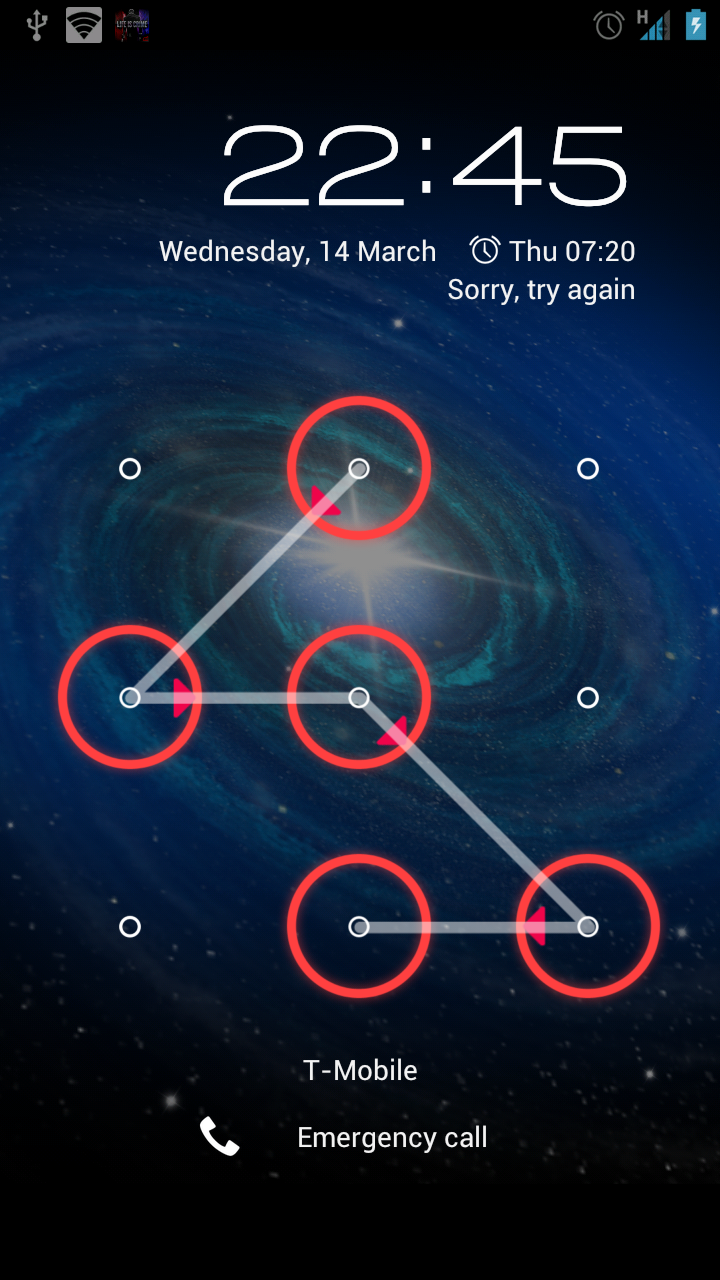
\includegraphics[scale=0.15]{pics/patternLock.png}
      \end{center}
      \vspace{-5pt}
      \caption{Usability vs. Security}
      \vspace{-10pt}
    \end{wrapfigure}
    
      \begin{itemize}
        \item None
        \item Swipe
        \item Face Recognition
        \item PIN code
        \item Pattern
        \item Password
      \end{itemize}
    
    The Android Unlock Patterns are a simplified version of the Pass-Go scheme that was proposed by Tao and Adams in 2008, and can be seen as a successor of the Draw-a-Secret (DAS) scheme. Both Pass-Go, Draw-a-Secret, and Android Unlock Patterns is categorized as recall-based authentication schemes.
    The Android password patterns are a simplified version of the Pass-Go scheme using a 3x3 grid, instead of a 9x9 as the Pass-Go scheme originally was designed. The Pass-Go scheme was inspired from the Chinese board game ``Go''.

    When the user first starts using the phone, they are prompted with the choise of using a locking mechanismn on the phone. The functionality of the Android Unlock Pattern are as follow: 
      \begin{enumerate}
        \item At least four points must be chosen,
        \item You cannot visit the same node twice.
        \item Only straight lines are allowed, and
        \item One cannot jump over point not visited before
      \end{enumerate}

  \section{Choice of Pattern Lock Functionality}

  \section{Success Criterias}

    When selecting method for colleting data it is essential to analyse and define success criteras to obtain good results in the data analysis that will be conducted in the following spring. 

    {\bf Target population:}
    {\bf Sampling plan:}
    {\bf Collection instruments:}
    

  \section{Data Collection Methods}

    When collecting data a design can use different methods that will influence the collected data and have different pros and cons. In this section we will look further into different variations, and choose the method that will support the studies success criterias. 


  \section{Ethical Consierations}





